% file: sections/bicomp-dfs-alg.tex

\documentclass[tikz]{standalone}
\usetikzlibrary{positioning, shapes}

\begin{document}
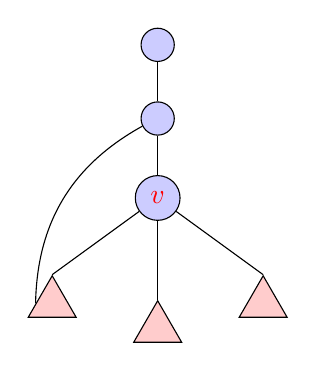
\begin{tikzpicture}[normal/.style = {circle, minimum size = 12pt, draw, fill = blue!20},
    subtree/.style = {regular polygon, regular polygon sides = 3, minimum size = 20pt, draw, fill = red!20},
    every edge/.style = {draw}] 
  \node (1) [normal] {};
  \node (2) [normal, below = 0.50cm of 1] {};
  \node (3) [normal, below = 0.50cm of 2] {\textcolor{red}{$v$}};

  \node (m) [subtree, below = of 3] {};
  \node (l) [subtree, below left = of 3] {};
  \node (r) [subtree, below right = of 3] {};

  \path (1) edge (2)
  	(2) edge (3)
	(3) edge (m)
	(3) edge (l.north)
	(3) edge (r.north)
	(l.west) edge[bend left] (2);
\end{tikzpicture}
\end{document}
